\documentclass[reprint,amsmath, amsfonts, amssymb, aps, letterpaper]{revtex4-1}

\usepackage{graphicx,float}
%\usepackage[caption=false]{subfig}
\usepackage{dcolumn}
\usepackage{bm}
\usepackage{enumitem}
\usepackage{tabularx}
\setlength{\extrarowheight}{6 pt}
\newcolumntype{Y}{>{\centering\arraybackslash}X}
\setlist[enumerate]{topsep=0pt,itemsep=-1ex,partopsep=1ex,parsep=1ex}
\usepackage{natbib}
\usepackage{physics}
\usepackage{fancyhdr}
\usepackage{amsthm}
\usepackage{amsmath}
\usepackage{graphicx}
\usepackage{amssymb}
\usepackage{esint}
\usepackage{color}
\usepackage{moreverb}
\usepackage{wrapfig}
\usepackage{physics}
\usepackage{siunitx}
\usepackage{subfig}
%\usepackage{wrapfig}


\begin{document}

\preprint{PHYS CS 15C}
\title{Remotely Operated Vehicle (ROV) with Touch Sensing Control}
\author{Menghang (David) Wang, Weiheng (Frank) Fu, Yiluo Li}
\affiliation{University of California, Santa Barbara, California 93107}

\date{\today}

% Intrigue your audience, connect your project with something people feel more interested in general

% to measure the systematic error, you can try best to maximize the potential one and see if it will genuinely have much effect

\begin{abstract}

\end{abstract}

\maketitle

\section{Introduction}
Often times there exist terrain on which people cannot tread on. Whether it be disaster debris or remote terrain such as Mars, it would provide much convenience if we are allowed to control the vehicle remotely while still being able to see directly how the terrain looks like. Under such circumstance, we wish to construct a robot that will follow our command on a model terrain that replicate the scale and feature of the actual terrain.
\\\indent To achieve such goal, we chose to create a touching pad sprayed with carbon conductive material, and scaled the size according to the dimension of the track on which our vehicle would be walking on. This served as our toy model for the remotely controlled vehicle on a visualized terrain. On the touching pad, we used electric sensing mechanism to measure the voltage drop across different locations, process the data to predict the finger location, and send the corresponding command through infrared to the vehicle.

\subsection{Setup overview}
\begin{figure}[h]
\centering
    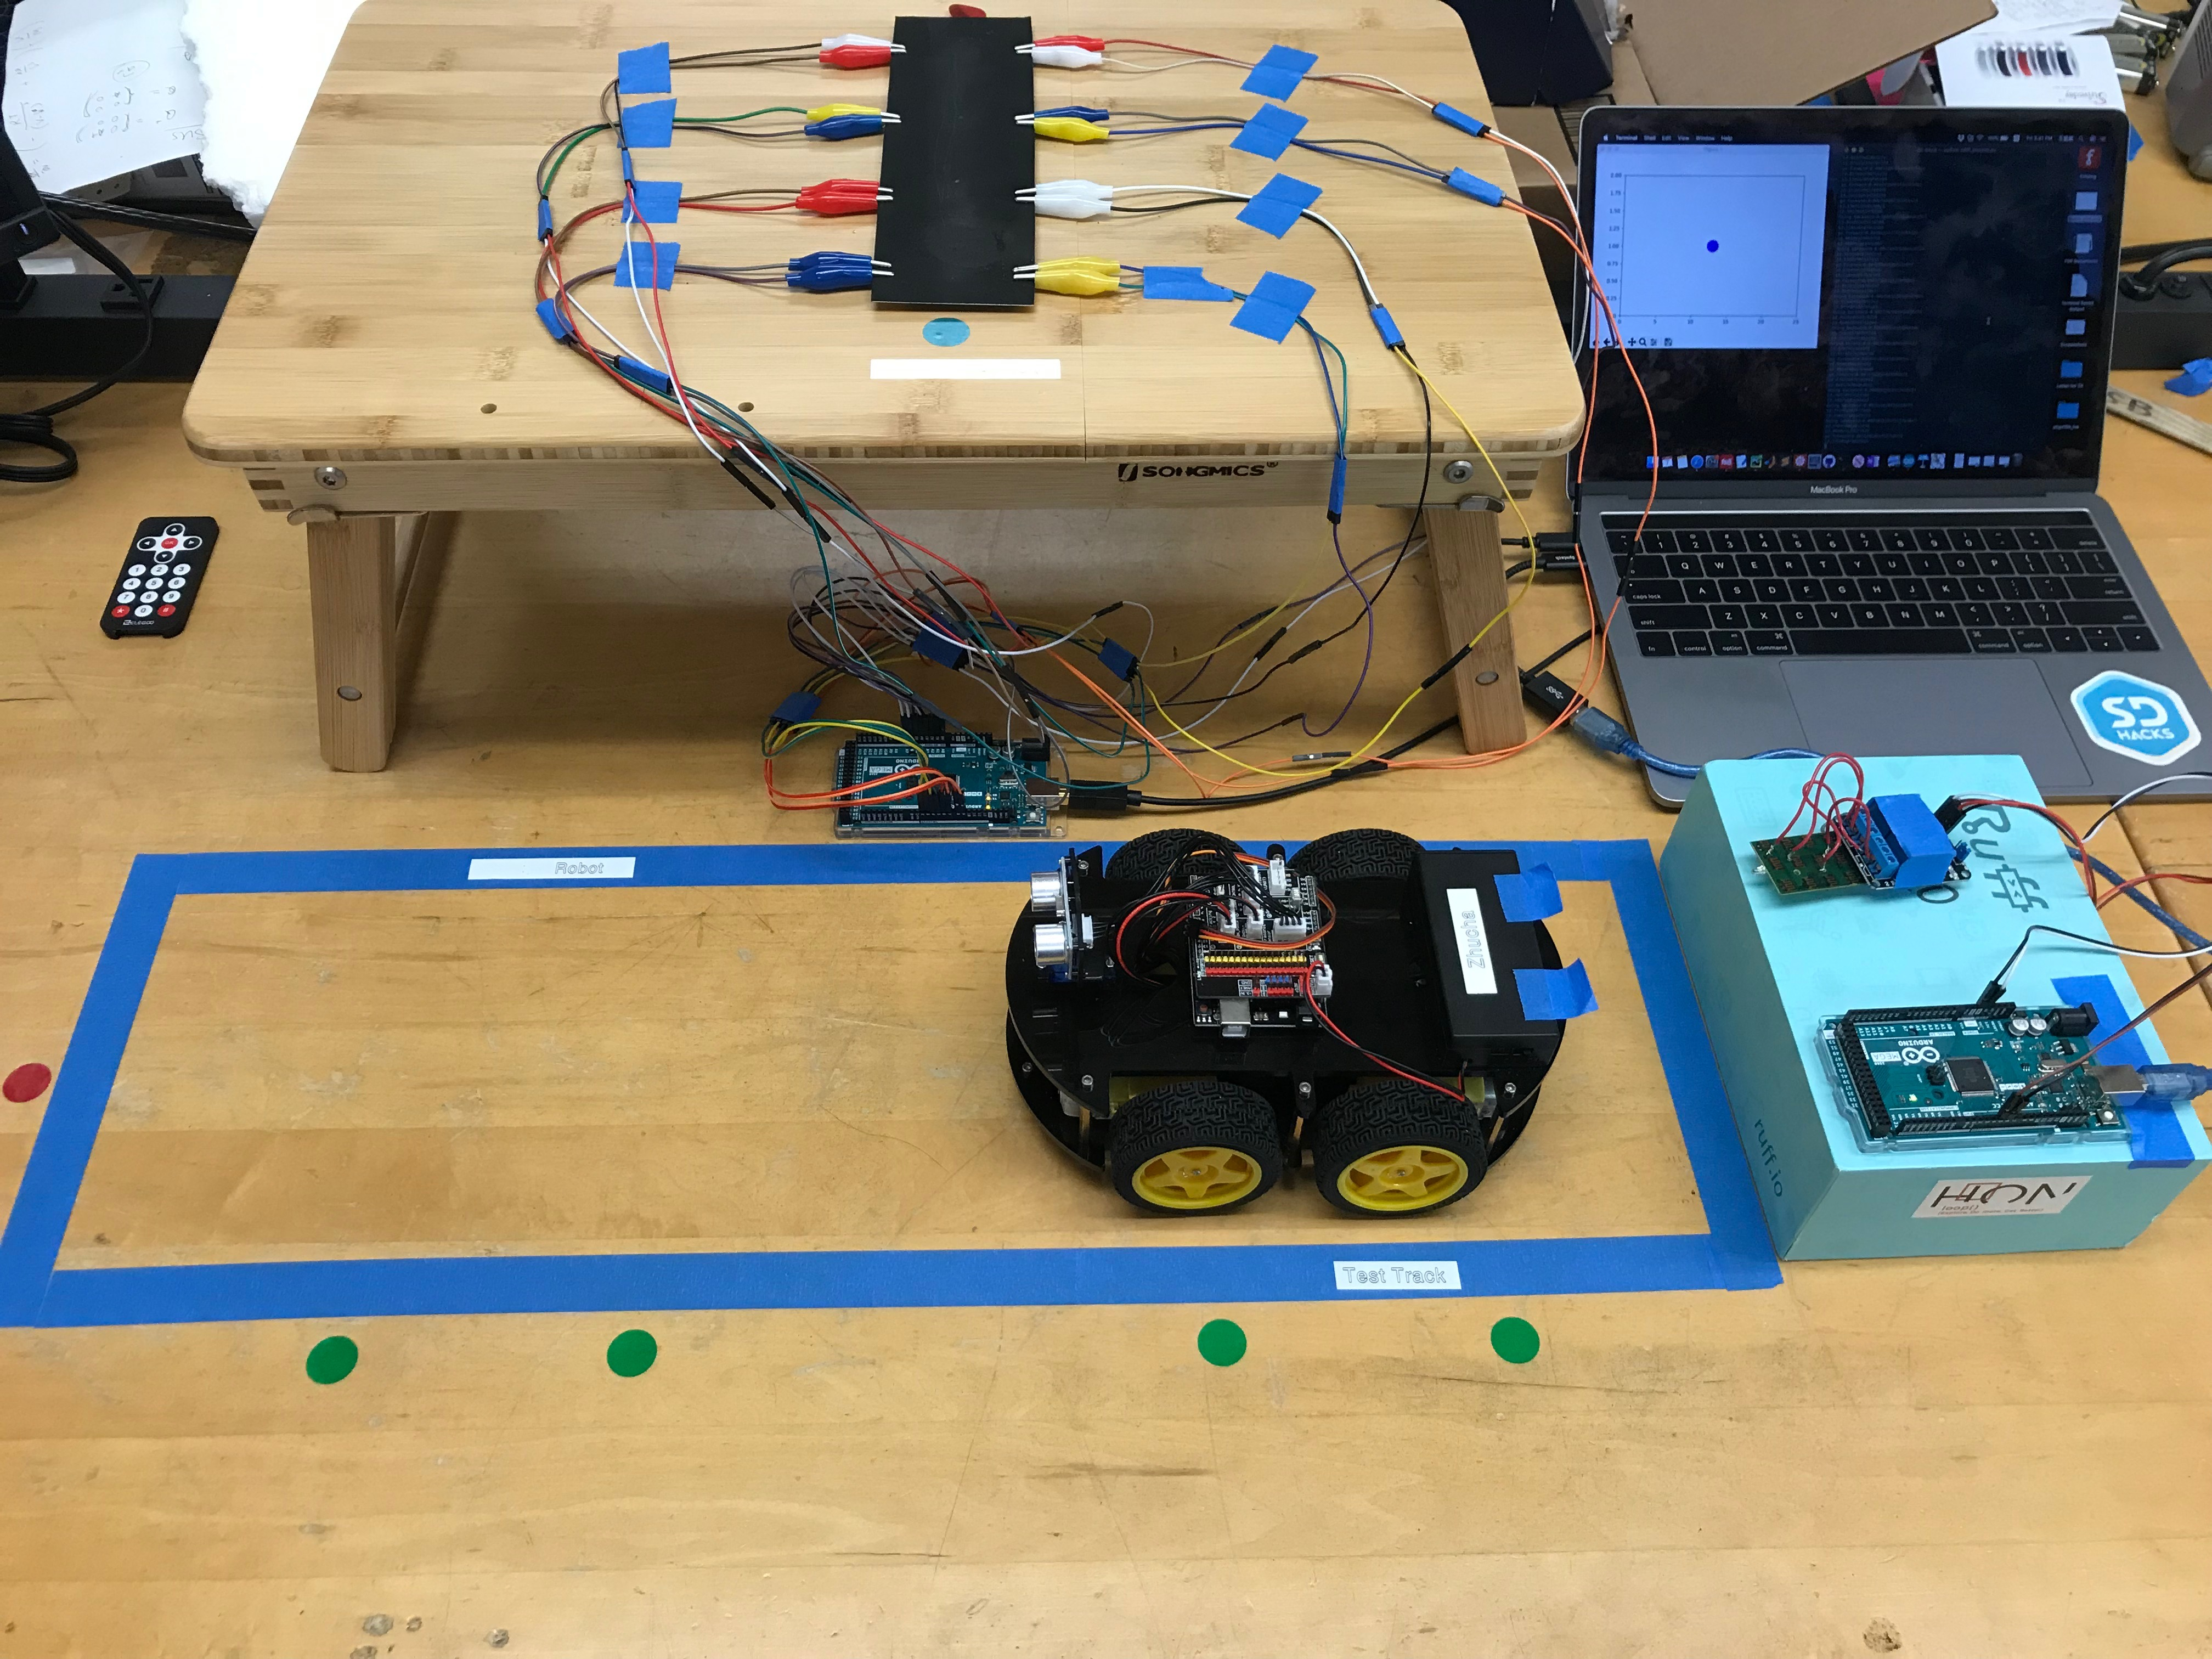
\includegraphics[width=0.4\textwidth]{./figure/setup}     
       \caption{Setup of ROV and touching pad }
    \label{fig::setup}
\end{figure}

\section{Touching Pad}
The goal of the touching pad is that it can be manufactured by shrinking the real size of the actual terrain where the ROV operates. Then, any touching on the touching pad will correspond to a real coordinate in the actual terrain. Therefore, the command applied on the touching pad will correspond to a command of the ROV in the real field. In this section, we are going to introduce the method we constructed the touching pad and the mechanism we use to sense the touch.


\section{Touching Pad}

\subsection{Electric sensing principle}
Our sensing principle is based on the a carbon-coated plastic board which changes its resistance distribution when the mechanical deformation happens on the board. We also call this method Dynamic Pressure Sensing since as we put our finger on the board, the contact pressure creates the local deformation on the board. This deformation leads to a change in the resistance distribution of the board. 

In Fig. \ref{fig::pressure}, DC current is used to describe the shift of voltage created by the pressing of the finger. When no pressure is applied on the material, the voltage stays constant, which we called baseline. As we may observe, the press of the finger cause an increase of the voltage. When we release the finger, the voltage drops back to the the line which is close to the initial voltage. However, one thing deserved notice is that the voltage does not drop back to the baseline exactly. This phenomenon introduces 3 \% error in this test but we did not consider its effect in our setup of the touching pad. We will discuss the issue in details in the section for future improvement.

\begin{figure}[h]
\centering
    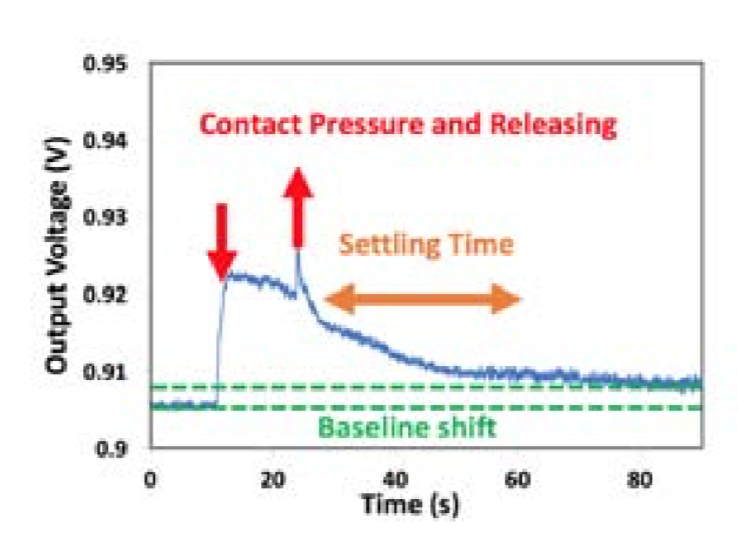
\includegraphics[width=0.45\textwidth]{./figure/pressure}     
       \caption{Voltage reading from a sensing channel fed with fixed DC current upon pressure. The green line (baseline) represent the voltage when no pressure is applied on the board, while the blue line describe the voltage shift caused by the pressing and releasing of the finger. \citep{isoft} }
    \label{fig::pressure}
\end{figure}

In addition, we also tried to implement another popular sensing mechanism based on electric shunting \cite{shunt}, which is implemented by Zhang \cite{electrick}. This mechanism is wildly utilized in Electric Field (EF) sensing systems \cite{ef}. However, this principle requires generating high frequency (200Khz) AC current and higher standard for noise reduction. The wave generator we used, Arduino Mega 2560 \citep{arduino}, cannot generate clean enough signal and the effect of electric shunting cannot be detected from the measurement. Hence, we choose to use the dynamic pressure sensing as our sensing principle.
\subsection{Touching pad setup}
The touching pad is constructed by spraying a conductive carbon paint made by MG Chemicals \citep{carbon} on the surface of a plastic board (25cm $\times$ 6cm). Eight electrodes are placed on the peripheral of the board with separation 6cm and each electrode is consist of 2 alligator clips with one of them applying the voltage and the other measures the voltage. Each 
\begin{figure}[h]
\centering
    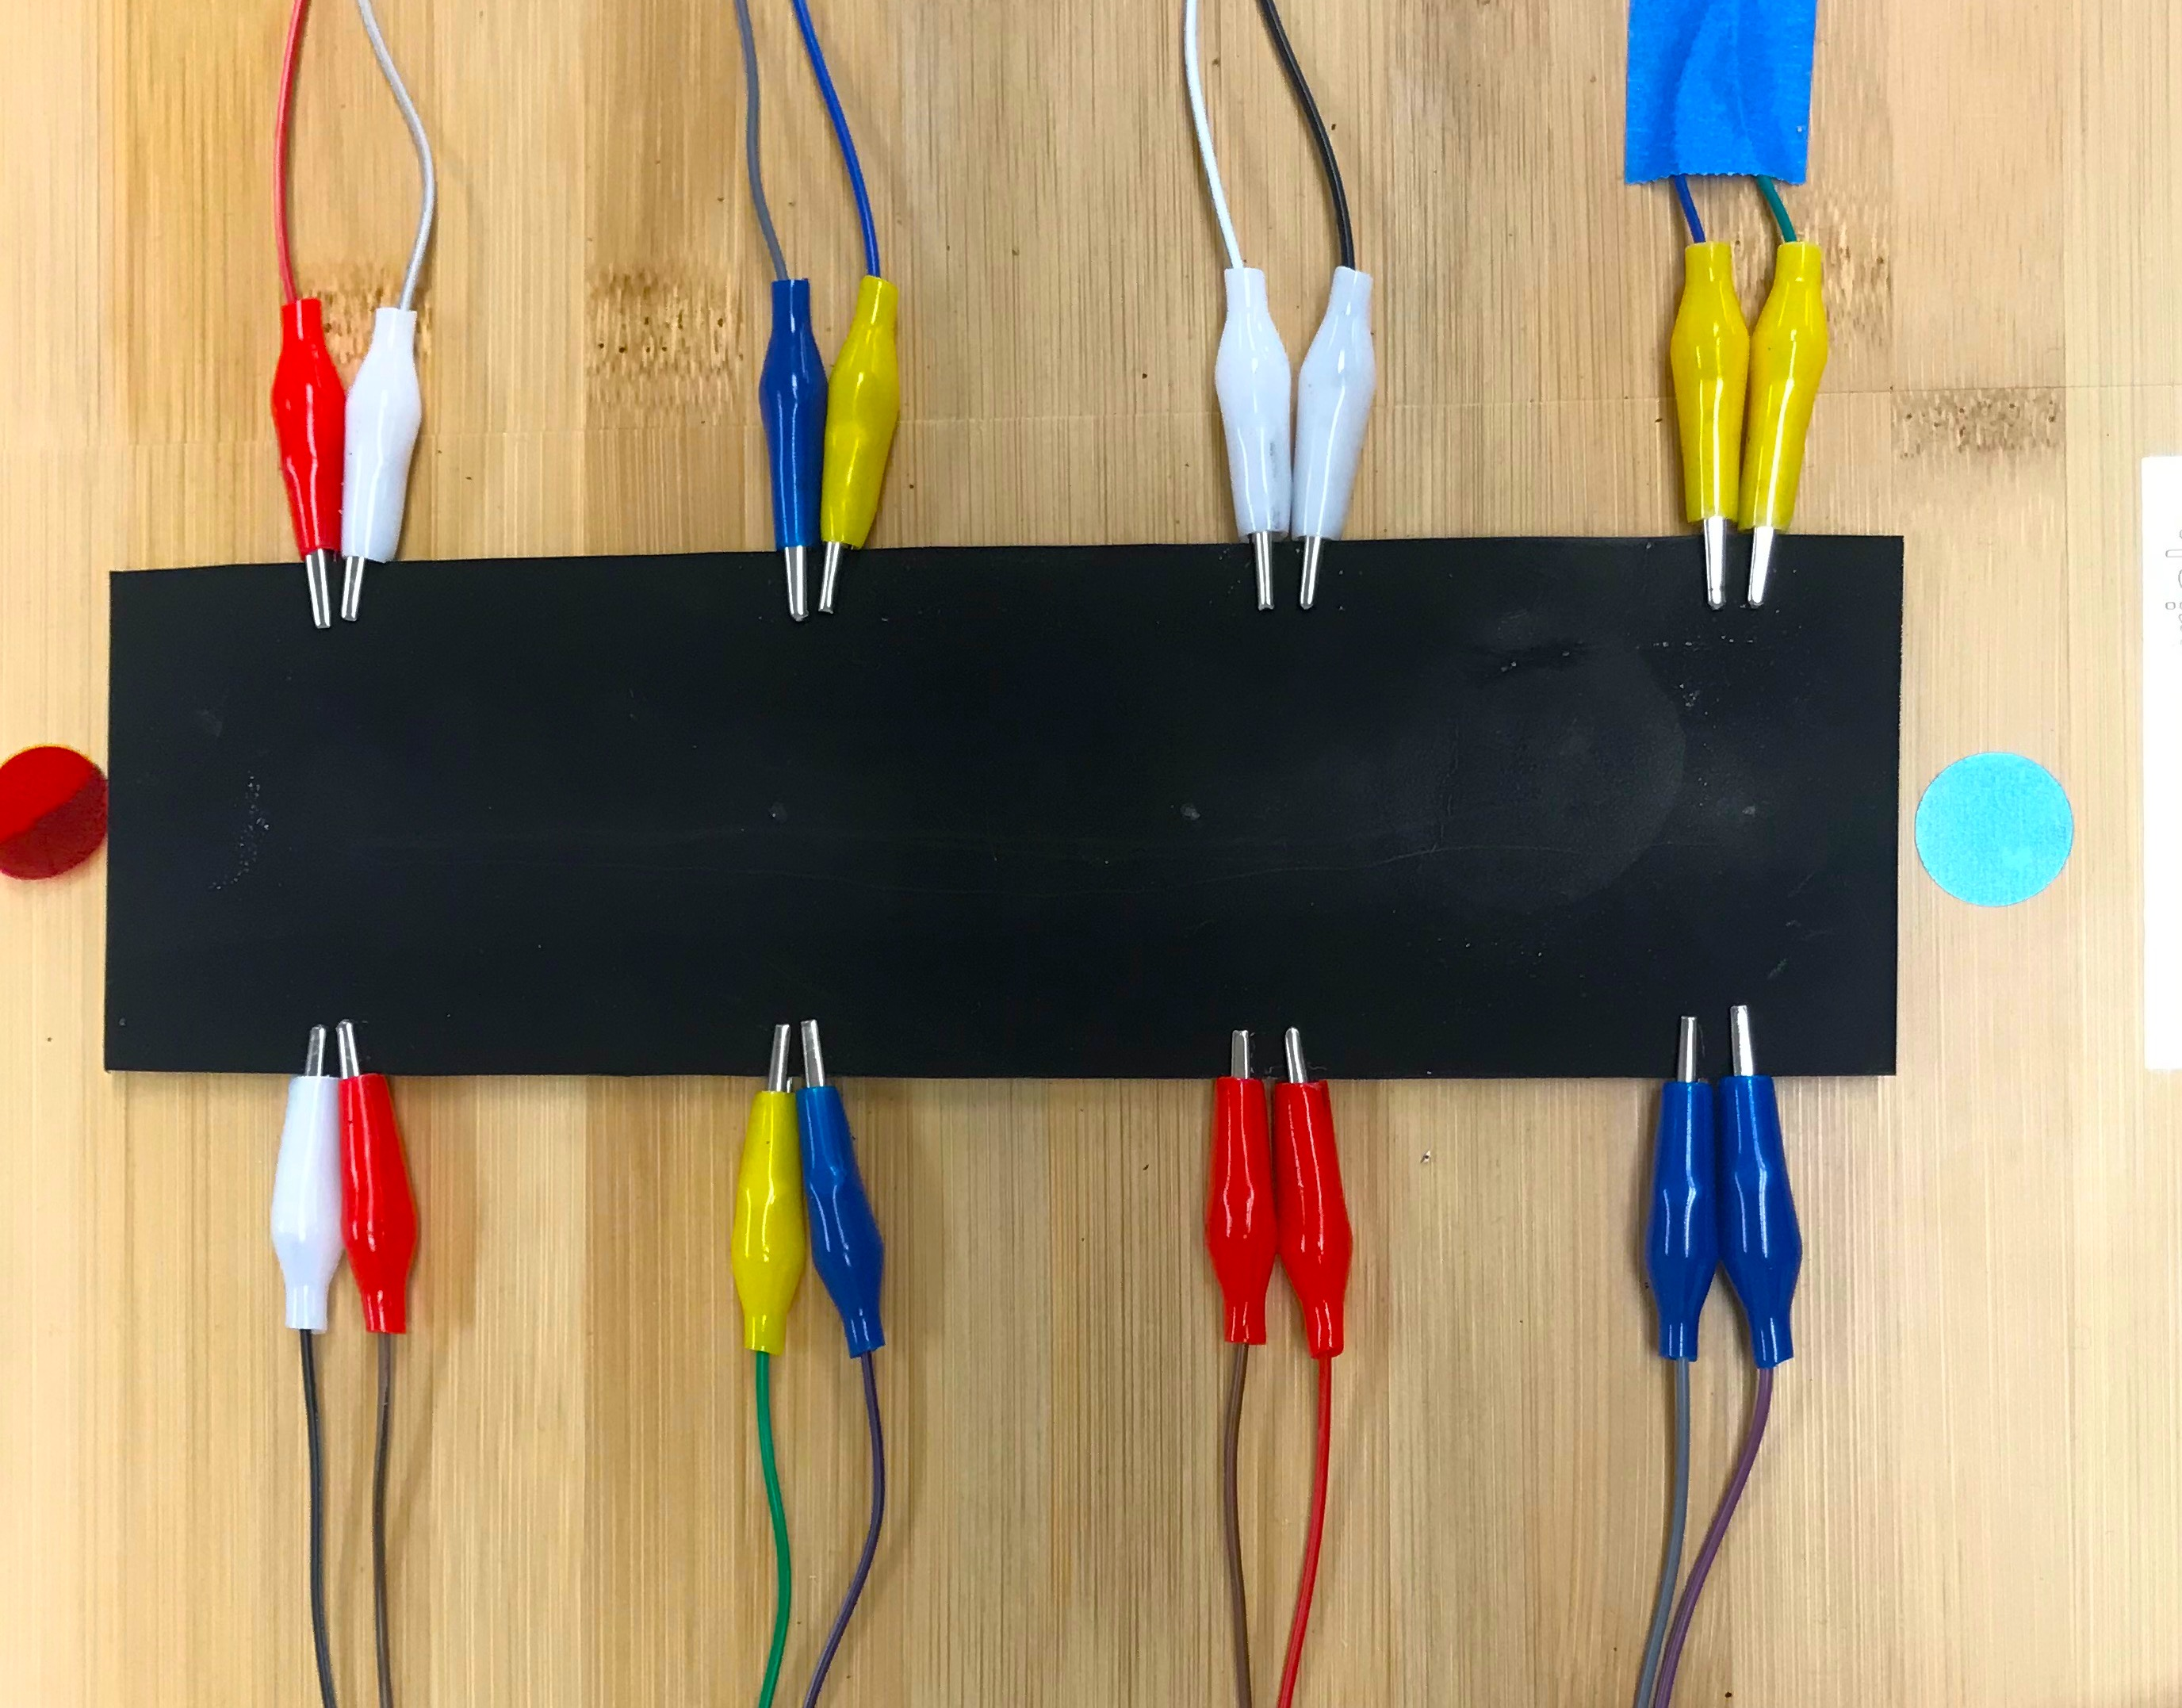
\includegraphics[width=0.45\textwidth]{./figure/pad}     
       \caption{. \citep{isoft} }
    \label{fig::pad}
\end{figure}
\subsection{Measuring procedures}
\subsection{Implementation}

\section{Visualization and Locating Finger}
\subsection{Voltage color-map}
To better monitor the performance of our voltage measurements, we created a real-time voltage map to visualize the data intake at each electrode. In order to see clearly the fluctuations, every time when we run the processing code, we would first run a round of measurement to initialize an offset value that would be subtracted from the later measurements. This is to help us magnify the variations of voltage around a certain value that is different every time due to the easily deformable nature of our touching pad.
\\\indent As we eventually ended using the rectangular touching pad for 1D control, we were aiming for distinguishing the finger locations at four different points. Previously the voltage drop patter could hardly be seen from the voltage map when we attempted to use a large rectangular touching pad. However, as we switched to the 1D touching pad, we could distinguish by eyes that by applying deformation at four different points, we would measure four distinct patterns of voltage drop across the electrodes, as seen in \ref{fig::voltage_map}
\begin{figure}
 	\subfloat[]{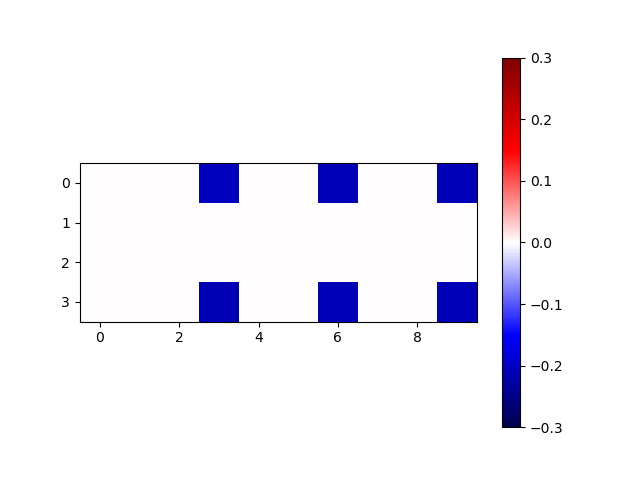
\includegraphics[scale=0.5]{figure/rec1}}\\
 	\subfloat[]{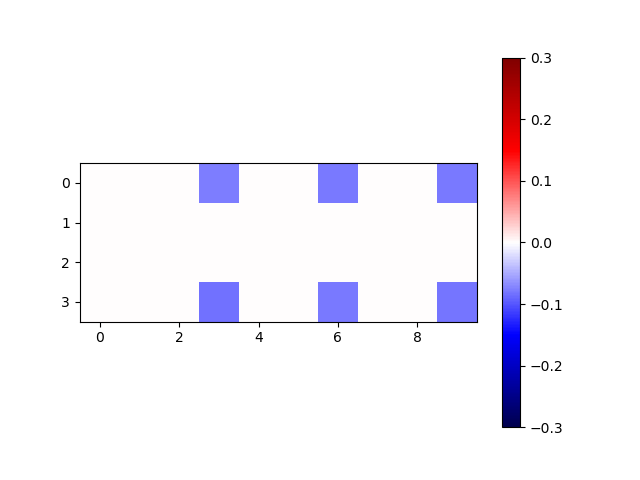
\includegraphics[scale=0.5]{figure/rec2}}\\
 	\subfloat[]{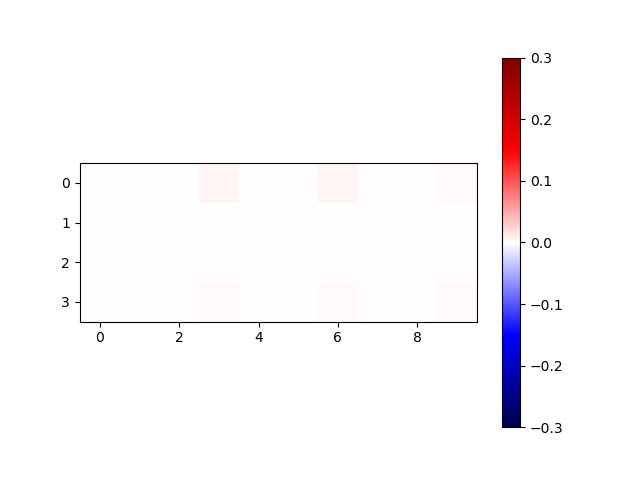
\includegraphics[scale=0.5]{figure/rec3}}\\
 	\subfloat[]{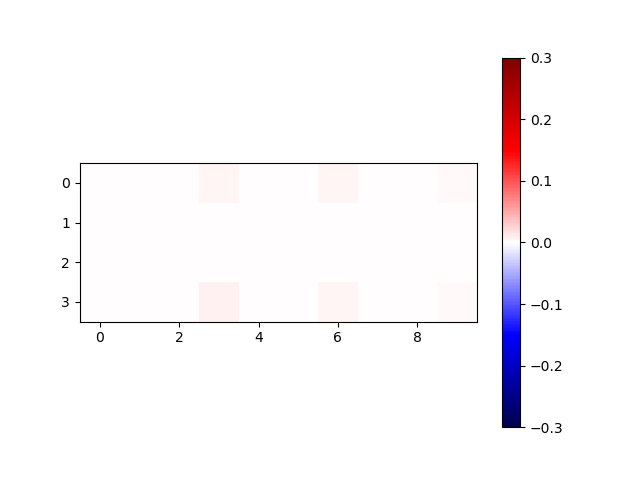
\includegraphics[scale=0.5]{figure/rec4}}
 	\caption{The visualization of voltage measurements when causing deformation at four middle points between opposite electrodes\label{fig::voltage_map}}
\end{figure}
 
\subsection{Locating finger with machine learning}

\begin{equation}
 	\theta = (X^TX)^{-1}(X^Ty)
\end{equation}

\section{Remotely Operated Robot (ROV)}
We assembled our robot using the components that were bought online. We programmed the robot so that it can be controlled by a pre-made infrared remote control. Instead of pushing physical buttons, the remote can be switched on and off by the relay, which is wired to an Arduino Mega connected to the computer. In the graph, the relay and remote is in the lower part connected together by blue tape.

\begin{figure}[!htb]
\begin{center}
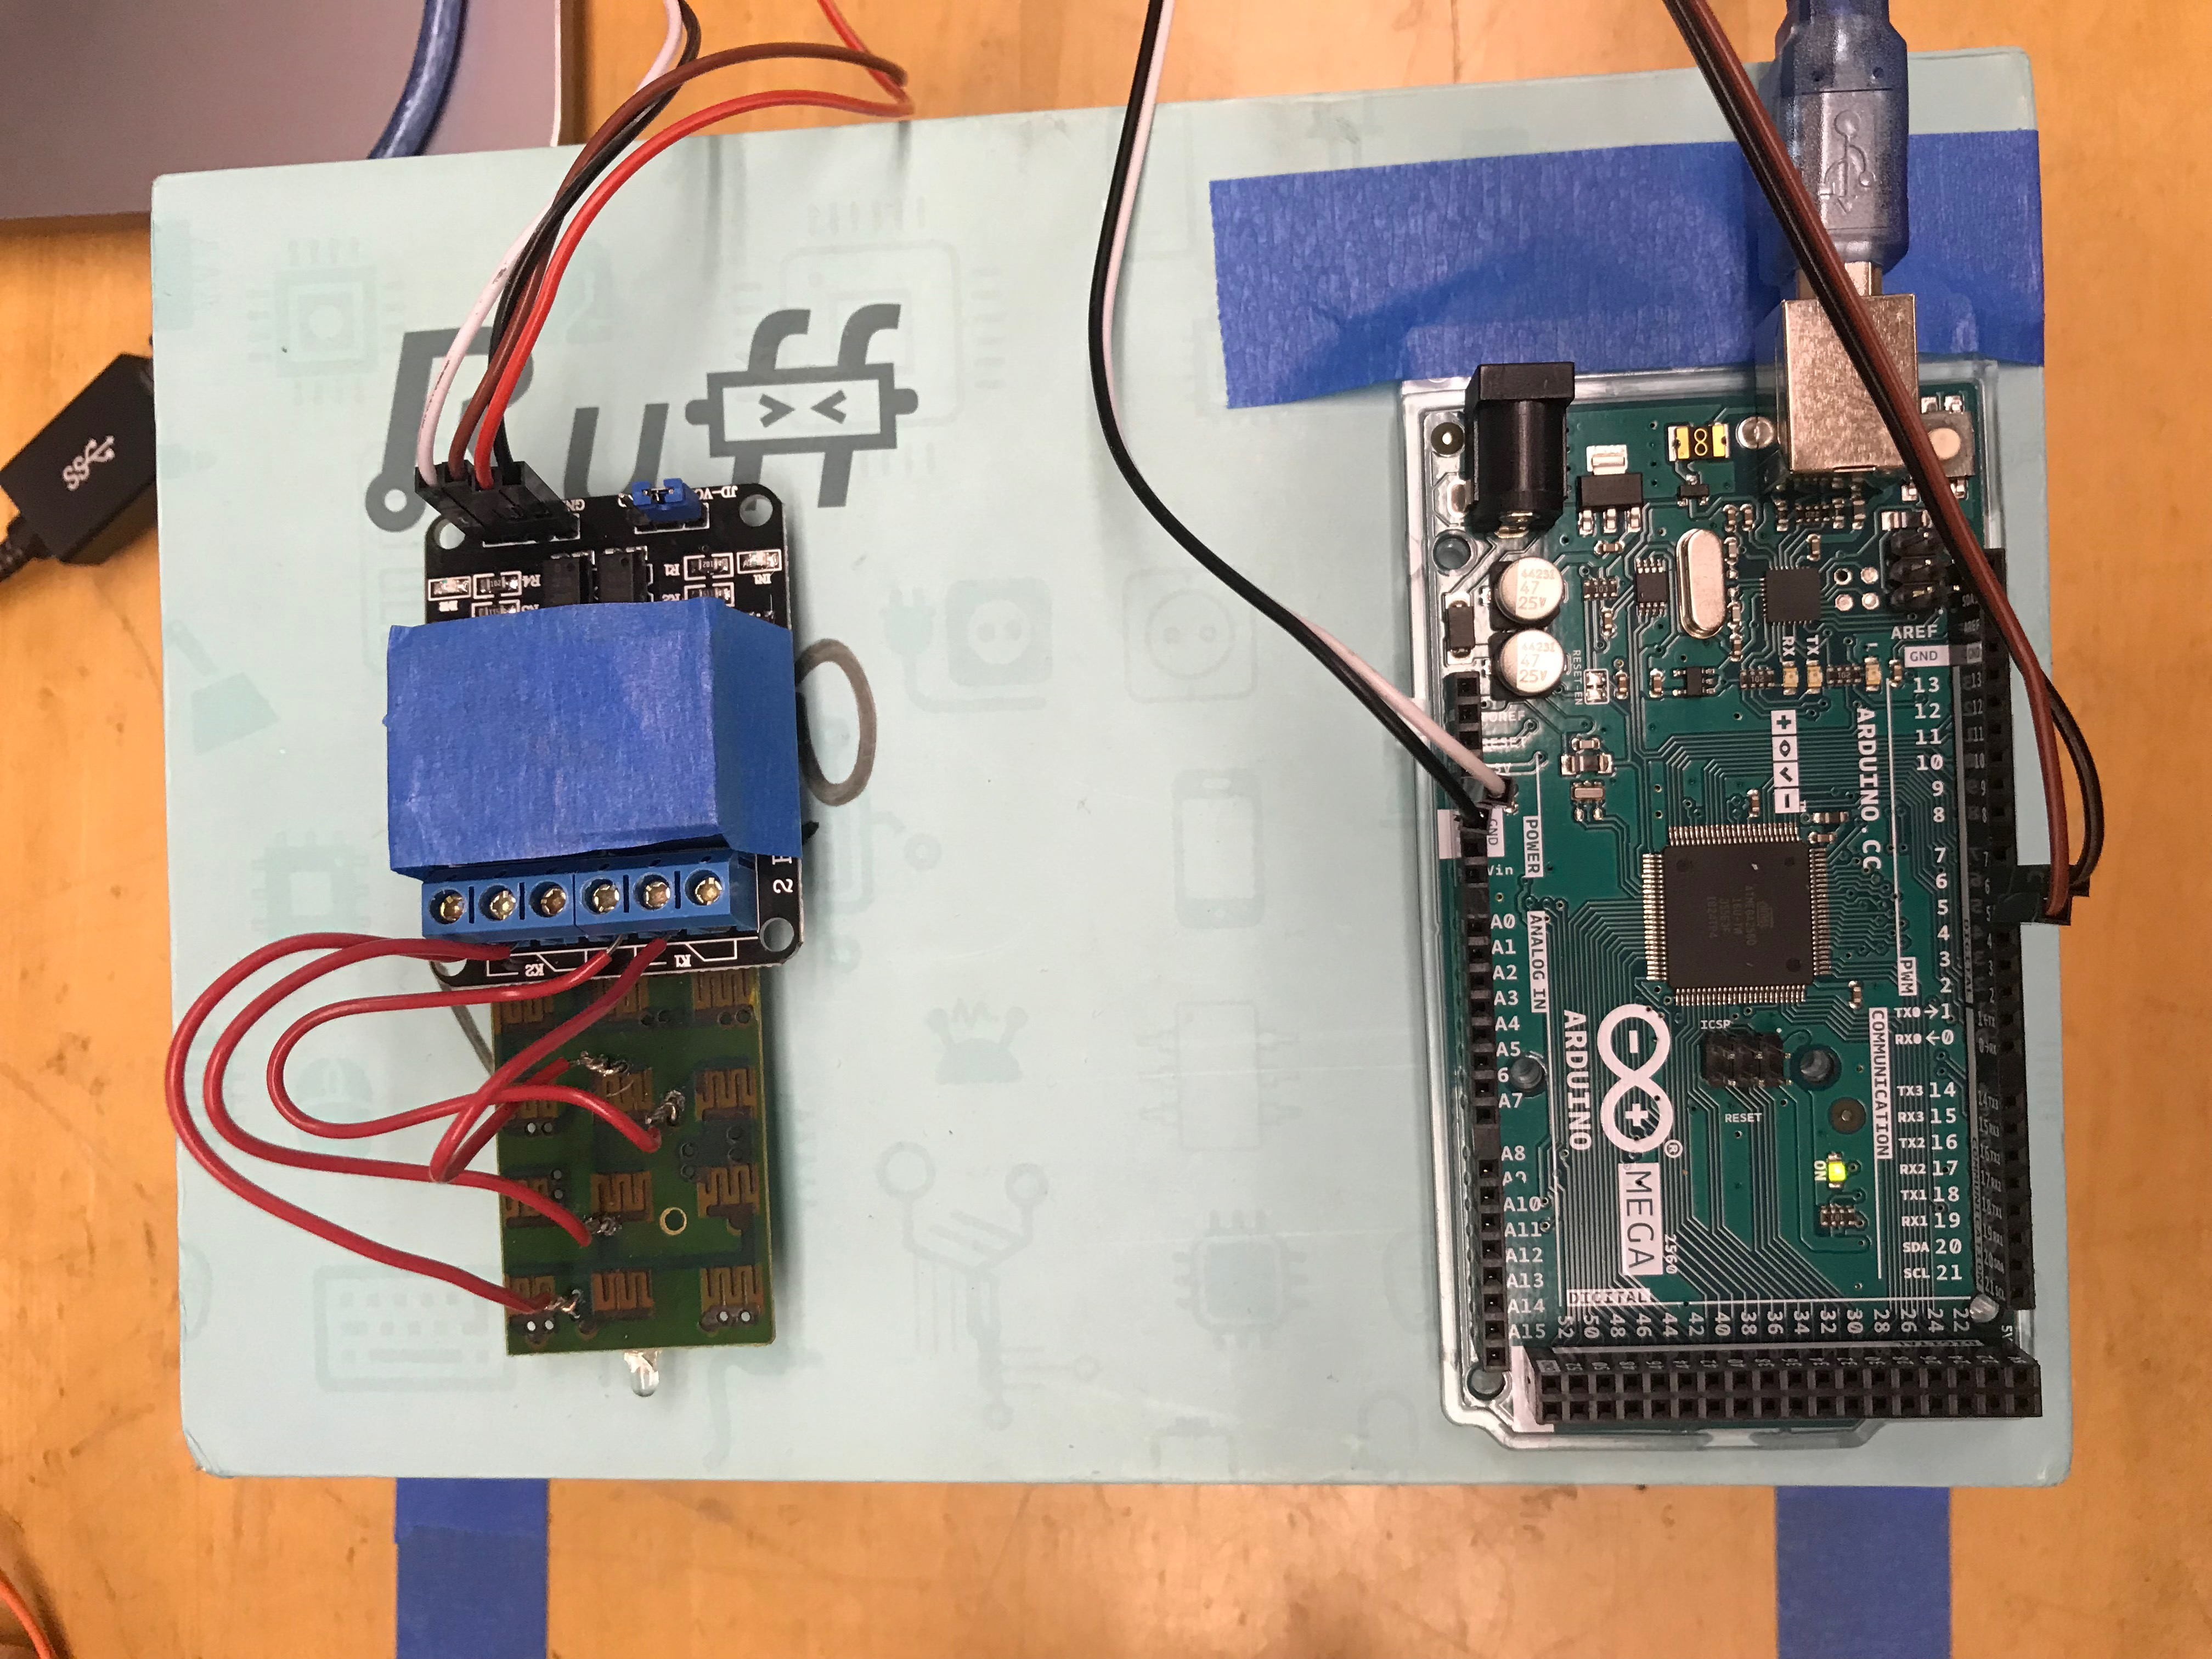
\includegraphics[width=3in]{relay.jpg}
\caption{Remote control, Relay, and Arduino Mega}
\label{fig1}
\end{center}
\end{figure}

\subsection{Modules}
Our robot is driven by four DC motors. Since we used a L298N dual full bridge driver, the motors of each side had to be wired together. To make the robot move slower, we have gear boxes connected to each of the motors. In addition, PWM is used instead of usual analog pins. We used Arduino Uno to control the whole robot, and mounted Vishley TSOP32238 infrared control on Uno. The power is provided by two 18650 lithium batteries. The robot also comes with other potentially useful components, such as line tracking module, ultrasonic sensor, and bluetooth module.

\subsection{Control method}
Initially we proposed to control the robot using bluetooth module, but after some time, we realized that bluetooth is not a great idea as it is hard to interface with python, not to mention dealing with the various protocols. As a result, we turned to a pre-made remote control instead. We used the relay to control the remote control and the distance robot travels can be monitored by changing the time duration that the remote is switched on. From many trials we found the distance traveled by robot and the remote's ON duration is not a strict linear relationship as we expected. 

As a result, some data is taken and it turns out there was a minimum distance the robot must move. One possible reason is that one complete infrared signal has a minimum required time to send depending on the string that is encoded. In this case, no matter how soon we make the time duration, at a certain point, the signal duration will not become shorter anymore. To resolve this issue, we set the PWM on the motor to the minimum possible (that is, any power lower than this will not be enough to move the robot).Thus, we successfully reduced the minimum distance to about 11.5 centimeters. We also did linear regression to find the correspondence of time and movement distance after minimal distance.

As the accuracy of our track pad is vertainly larger than 1 cm, and the track pad is 23 cm long, we just set the ratio between touch pad and robot movement as 1:11.5 to eliminate the issue. Now this error is acceptable since track pad is now a larger error source.

Some drawbacks of this method is that there is really no feedback, so we were unable to do error control. If we had more time, some possible solutions would be: \\
1) change DC motors into stepper motors, \\
2) build a custom infrared remote so we can directly tell the robot how long to travel, and \\
3) use ultrasonic sensor as a means of feedback.
\subsection{Communication with the touching pad}


\section{Future Improvement}
\subsection{•}

We used a protocol called pyFirmata to communicate with Arduino from our computer using python. After the individual robot control program is debugged and tested, we integrated it into our main program.


\nocite{*}
\bibliography{rov}% Produces the bibliography via BibTeX.

\end{document}



